\documentclass{article}

\usepackage{fullpage}
\usepackage{url}
\usepackage{graphicx}
\usepackage{amsmath}
\usepackage{physics}
\usepackage{mathtools}

\DeclareMathOperator{\erfi}{erfi}
\newcommand{\R}{\ensuremath{\mathbb{R}}}

\title{Quantum Mechanics I Excercise 3}
\author{Idan Stark}
\date{\today}

\begin{document}
\maketitle

\section{The semiclassical limit for momentum space path integral}
\subsection{Classical equations and boundary conditions}
Following the same method in the notes, we start from the path integrals in phase space formulation:
\begin{equation}
    K(x_f, t_f : x_i, t_i) = \int Dx(t) Dp(t) \exp[\frac{i}{\hbar}S\left[p(t), x(t)\right]]
\end{equation}
With the action
\begin{equation}
    S\left[p(t), x(t)\right] = \int_{t_i}^{t_f} dt \left[p(t) \frac{dx(t)}{dt} - H(p(t), x(t))\right]
\end{equation}
Since we want this in the momentum space:
\begin{equation}
\begin{gathered}
    K(p_f, t_f : p_i, t_i) = \bra{p_f}U(t_f, t_i)\ket{p_i} =
    \int dx_i dx_f \bra{p_f}\ket{x_f}\bra{x_f}U(t_f, t_i)\ket{x_i}\bra{x_i}\ket{p_i} =
    \\
    = \frac{1}{2\pi\hbar}\int dx_i dx_f e^{-ip_fx_f/\hbar}K(x_f, t_f : x_i, t_i)e^{ip_ix_i/\hbar} =
    \\
    = \frac{1}{2\pi\hbar}\int dx_i dx_f e^{\frac{i}{\hbar}(p_ix_i - p_fx_f)}K(x_f, t_f : x_i, t_i)
    \\
    = \frac{1}{2\pi\hbar}\int Dx(t) Dx(t) \exp[\frac{i}{\hbar}\left(S\left[p(t), x(t)\right] + p_ix_i - p_fx_f\right)]
\end{gathered}
\end{equation}
The object in the exponent can be simplified by integrating by parts the $p\dot{x}$ in the action:
\begin{equation}
\begin{gathered}
\label{eq:first-action}
    \tilde{S}\left[p(t), x(t)\right] = S\left[p(t), x(t)\right] + p_ix_i - p_fx_f =
    \\
    = \int_{t_i}^{t_f} dt \left[p(t) \frac{dx(t)}{dt} - H(p(t), x(t))\right] + p_ix_i - p_fx_f = 
    \\
    = \int_{t_i}^{t_f} dt \left[-x(t) \frac{dp(t)}{dt} - H(p(t), x(t))\right]
\end{gathered}
\end{equation}
In the limit $\hbar \rightarrow 0$, the stationary solutions will dominate the integral, which will happen when the exponent is zero:
\begin{equation}
    \delta \tilde{S} = 0
\end{equation}
We can look at the object inside the time integral as a lagrangian, and so the EOMs that stem from the minimization of the integral are the E-L equations for $x$ and $p$. In other words, in the phase space $x$ and $p$ are two coordinates of this lagrangian, so we can perform E-L equation for each of them. We will get to the canonical relations:
\begin{equation}
\label{eq:canonical-relations}
    \frac{dx_{cl}(t)}{dt} = \left.\frac{\partial H(p(t),x(t))}{\partial p(t)}\right|_{p=p_{cl}, x=x_{cl}}
    \qquad
    \frac{dp_{cl}(t)}{dt} = -\left.\frac{\partial H(p(t),x(t))}{\partial x(t)}\right|_{p=p_{cl}, x=x_{cl}}
\end{equation} 
Finally, since the path is between predetermined momentum states, they will give the boundary conditions:
\begin{equation}
\begin{gathered}
    p_{cl}(t_i) = p_i \qquad p_{cl}(t_f) = p_f
\end{gathered}
\end{equation}
\subsection{The Gaussian Integral}
Similarly to the coordinate space derivation, we will define the diviation from the classical momentum:
\begin{equation}
    p(t) = p_{cl}(t) + q(t)
\end{equation}
With the boundary conditions
\begin{equation}
    q(t_i) = q(t_f) = 0
\end{equation}
And a diviation from the classical path:
\begin{equation}
    x(t) = x_{cl} + y(t)
\end{equation}
Without boundary conditions.
We can now rewrite the path integral as
\begin{equation}
\begin{gathered}
    K(p_f, t_f : p_i, t_i) = \frac{1}{2\pi\hbar}\int Dx(t) Dp(t) \exp[\frac{i}{\hbar}\tilde{S}[p(t), x(t)]] =
    \\
    = \frac{1}{2\pi\hbar} \exp[\frac{i}{\hbar}\tilde{S}[p_{cl}(t),x_{cl}(t)]] \int Dx(t) Dp(t) \exp[\frac{i}{\hbar}\left(\tilde{S}[p(t),x(t)] - \tilde{S}[p_{cl}(t),x_{cl}(t)]\right)] =
    \\
    = F(p_f, t_f : p_i, t_i) \exp[\frac{i}{\hbar}\tilde{S}[p_{cl}(t),x_{cl}(t)]] 
\end{gathered}
\end{equation}
Which means
\begin{equation}
    F(p_f, t_f : p_i, t_i) = \frac{1}{2\pi\hbar} \int Dx(t) Dp(t) \exp[\frac{i}{\hbar}\left(\tilde{S}[p(t), x(t)] - \tilde{S}[p_{cl}(t), x_{cl}(t)]\right)]
\end{equation}
Expanding $\tilde{S}[p(t),x(t)]$ around $p_{cl}(t)$ and $x_{cl}(t)$, and remembding that still $\delta\tilde{S} = 0$, we get
\begin{equation}
\label{eq:basic_action_diviation}
    \tilde{S}[p(t), x(t)] = \tilde{S}[p_{cl}(t), x_{cl}(t)] + \frac{1}{2}\delta^2\tilde{S}[q(t), y(t)] + O(\delta^3\tilde{S}[q(t),y(t)])
\end{equation}
To find the value of the second variation $\delta^2\tilde{S}[q(t)]$ we need to similarly expand the Hamiltonian. In the following calculation we leave the time dependence implicit:
\begin{equation}
\begin{gathered}
    H(p,x) = H(p_{cl}, x_{cl}) +
        \left.\frac{\partial H}{\partial x}\right|_{p=p_{cl}, x=x_{cl}}y + \left.\frac{\partial H}{\partial p}\right|_{p=p_{cl}, x=x_{cl}}q +
        \\
        +  \left.\frac{1}{2}\frac{\partial^2 H}{\partial x^2}\right|_{p=p_{cl}, x=x_{cl}}y^2
        +  \left.\frac{\partial^2 H}{\partial x\partial p}\right|_{p=p_{cl}, x=x_{cl}}yq
        +  \left.\frac{1}{2}\frac{\partial^2 H}{\partial p^2}\right|_{p=p_{cl}, x=x_{cl}}q^2 + O(\partial^3 H) = 
        \\
        \\
        = H(p_{cl}, x_{cl}) -
        \dot{p}_{cl}y + \dot{x}_{cl}q +
        \\
        +  \left.\frac{1}{2}\frac{\partial^2 H}{\partial x^2}\right|_{p=p_{cl}, x=x_{cl}}y^2
        +  \left.\frac{\partial^2 H}{\partial x\partial p}\right|_{p=p_{cl}, x=x_{cl}}yq
        +  \left.\frac{1}{2}\frac{\partial^2 H}{\partial p^2}\right|_{p=p_{cl}, x=x_{cl}}q^2 + O(\partial^3 H)
\end{gathered}
\end{equation}
We can now open the first part of the exponent using the diviations:
\begin{equation}
\begin{gathered}
    \int_{t_i}^{t_f} -x\dot{p} dt = -\int_{t_i}^{t_f} \left[x_{cl} + y\right]\left[\dot{p}_{cl} + \dot{q}\right] dt
    = -\int_{t_i}^{t_f} x_{cl}\dot{p}_{cl} + y\dot{p}_{cl} + x_{cl}\dot{q} + y\dot{q} dt =
    \\
    = -\left[x_{cl}q\right]_{t_i}^{t_f}-\int_{t_i}^{t_f} x_{cl}\dot{p}_{cl} + y\dot{p}_{cl} - \dot{x}_{cl}q + y\dot{q} dt
    = -\int_{t_i}^{t_f} x_{cl}\dot{p}_{cl} + y\dot{p}_{cl} - \dot{x}_{cl}q + y\dot{q} dt
\end{gathered}
\end{equation}
Where in the last transition we used the fact that $q(t_i) = q(t_f) = 0$.
These two equation mean that:
\begin{equation}
\begin{gathered}
    \tilde{S}\left[p(t),x(t)\right] = -\int_{t_i}^{t_f} dt \left[ x_{cl}\dot{p}_{cl} + y\dot{p}_{cl} - \dot{x}_{cl}q + y\dot{q} + H(p_{cl}, x_{cl}) -
    \dot{p}_{cl}y + \dot{x}_{cl}q + \right. + y\dot{q}
    \\ \left.
    +  \left.\frac{1}{2}\frac{\partial^2 H}{\partial x^2}\right|_{p=p_{cl}, x=x_{cl}}y^2
    +  \left.\frac{\partial^2 H}{\partial x\partial p}\right|_{p=p_{cl}, x=x_{cl}}yq
    +  \left.\frac{1}{2}\frac{\partial^2 H}{\partial p^2}\right|_{p=p_{cl}, x=x_{cl}}q^2 + O(\partial^3 H) \right]
    = \\ = \tilde{S}\left[p_{cl}(t), x_{cl}(t)\right] - \int_{t_i}^{t_f} dt y\dot{q} + \left[\left.\frac{1}{2}\frac{\partial^2 H}{\partial x^2}\right|_{p=p_{cl}, x=x_{cl}}y^2
    +  \left.\frac{\partial^2 H}{\partial x\partial p}\right|_{p=p_{cl}, x=x_{cl}}yq
    +  \left.\frac{1}{2}\frac{\partial^2 H}{\partial p^2}\right|_{p=p_{cl}, x=x_{cl}}q^2\right] + O(\delta^3\tilde{S})
\end{gathered}
\end{equation}
Comparing this to equation \ref{eq:basic_action_diviation}, it's clear to see that
\begin{equation}
\begin{gathered}
    \frac{1}{2}\delta^2\tilde{S}[q(t), y(t)] = - \int_{t_i}^{t_f}  y\dot{q} + \left.\frac{1}{2}\frac{\partial^2 H}{\partial x^2}\right|_{p=p_{cl}, x=x_{cl}}y^2
        +  \left.\frac{\partial^2 H}{\partial x\partial p}\right|_{p=p_{cl}, x=x_{cl}}yq
        +  \left.\frac{1}{2}\frac{\partial^2 H}{\partial p^2}\right|_{p=p_{cl}, x=x_{cl}}q^2dt
\end{gathered}
\end{equation}
\subsection{Finding $F$ and the Van-Vleck determinant}
Classically, propagating from a given initial momentum $p_i$ at time $t_i$ to a given final momentum $p_f$ at time $t_f$ requires a certain $x_i$ at time $t_i$. Changing the final momentum requires changing the initial position. Expanding around the classical solution, using the constant probability density for $x$ at a given momentum $\omega(x) dx_i = dx_i / 2\pi\hbar$, the probability to propagate into some momentum interval, $p_f < p < p_f + dp_f$ at $t_f$ will be, by the definition of the propagator,
\begin{equation}
    \left| K(p_f, t_f ; p_i, t_i)\right|^2dp_f = \frac{1}{2\pi\hbar} dx_i = \frac{1}{2\pi\hbar}\frac{dp_f}{\left|dp_f/dx_i\right|}
\end{equation}
And so, the semiclassical amplitude $F$ is
\begin{equation}
    \left|F(p_f, t_f; p_i, t_i)\right| = \frac{1}{\sqrt{2\pi\hbar\left|dp_f/dx_i\right|}} = \frac{1}{\sqrt{2\pi\hbar}}\sqrt{\frac{dx_i}{dp_f}}
\end{equation}
Since the exponent follows the canonical relations in equation \ref{eq:canonical-relations}, we can say that
\begin{equation}
    x_i = \frac{\partial \tilde{S}}{\partial p_i}
\end{equation}
This can also be seen from equation \ref{eq:first-action}
\begin{equation}
    \frac{\partial \tilde{S}}{\partial p_i} = 
    \frac{\partial}{\partial p_i} \left[\int_{t_i}^{t_f} dt \left[p(t) \frac{dx(t)}{dt} - H(p(t), x(t))\right] + p_ix_i - p_fx_f\right] = 
    x_i
\end{equation}
And so
\begin{equation}
    \left|F(p_f, t_f; p_i, t_i)\right| = \frac{1}{\sqrt{2\pi\hbar}}\sqrt{\frac{\partial^2 \tilde{S}}{\partial p_i\partial p_f}}
\end{equation}
Generalizing this to multiple dimensions is simple:
\begin{equation}
    \left| K(p(t_f), t_f ; p(t_i), t_i)\right|^2 \prod_{k=1}^M dx_k(t_f) = \prod_{n=1}^M 2\pi\hbar dp_n(t_i) = \det\left[\frac{\partial p_k(t_f)}{\partial x_n(t_i)}\right] \prod_{n=1}^M dx_n(t_i)
\end{equation}
Finally, using the opposite determinant rule $(\det P)^{-1} = \det (P^{-1})$ and again the canonical relations $x_n(t_i) = \frac{\partial \tilde{S}}{\partial p_n(t_i)}$:
\begin{equation}
    \left|F(p(t_f), t_f, p(t_i), t_i)\right| = \frac{1}{\left(2\pi\hbar\right)^{M/2}\sqrt{\det\left[\partial p_k(t_f)/\partial x_n (t_i)\right]}} = \frac{1}{\left(2\pi\hbar\right)^{M/2}}\sqrt{\det \left|\frac{\partial^2 \tilde{S}}{\partial p_k(t_f)\partial p_n(t_i)}\right|}
\end{equation}
\subsection{The Green's Function}
The Energy dependent Green's function's relation to the propagator in the phase space can be written as
\begin{equation}
    G(p_f,p_i;E) = \frac{1}{i\hbar}\int_0^\infty dT K\left(p_f,T;p_i,0\right)e^{iET/\hbar} = \frac{1}{i\hbar}\int_0^\infty dT F\left(p_f,T;p_i,0\right)e^{i\left(ET + \tilde{S}\left[p_{cl},x_{cl}\right]\right)/\hbar}
\end{equation}
For a classical trajectory $\hbar \rightarrow 0$, we can again use the stationary phase method, and require the derivative of the exponent by $T$ to be zero:
\begin{equation}
    E = -\frac{\partial \tilde{S}[p_{cl},x_{cl}]}{\partial T}
\end{equation}
Using equation \ref{eq:first-action} for a classical path, we get
\begin{equation}
    E = -\frac{\partial}{\partial T}
        \int_0^T dt \left[-x(t) \frac{dp(t)}{dt} - H(p(t), x(t))\right] = \frac{\partial}{\partial T}\left(\int_{p_i}^{p_f}xdp + E_{cl} T\right) = E_{cl}
\end{equation}
Which makes the expression in the exponent in the formula for the Green's function
\begin{equation}
    W(p_f, p_i ; E) = ET + \tilde{S}\left[p_{cl},x_{cl}\right] = ET - \left(\int_{p_i}^{p_f}xdp - E_{cl} T\right) = - \int_{p_i}^{p_f}xdp
\end{equation}
Which makes the stationary phase approximation of the Green's function
\begin{equation}
    G(p_f, p_i;E) \approx F(p_f, T(E); p_i, 0)\left(\frac{2\pi}{i\hbar \gamma(E)}\right)^{1/2}e^{i W(p_f, p_i ; E)/\hbar}
\end{equation}
Where
\begin{equation}
    \gamma(E) = \left.\frac{\partial^2 W}{\partial T^2}\right|_{T(E)} = \left.\frac{\partial E_{cl}}{\partial T}\right|_{T(E)}
\end{equation}

\section{Tunneling in momentum space}
\subsection{Classical trajectories with energy below the barrier}
For a one dimensional barrier, the constant energy lines in the phase space look like
\begin{equation}
    E = \frac{p^2}{2m} + V(x)
\end{equation}
where $E$ is constant. This means we can get two plots
\begin{equation}
\label{eq:classical-momentum}
    p = \pm 2m \sqrt{E - V(x)}
\end{equation}
Where the sign signifies the direction of motion. For a barrier with width $A$ of the structure
\begin{equation}
    V(x) = \begin{cases}
        \varphi(x) & |x| < A / 2 \\
        0 & else
    \end{cases}
\end{equation}
Where $\varphi(x)$ is some positive function for which $E < \varphi_{max} = V_{max}$. The equal-energy line in the phase space is split into two trajectories, each matching a different side of the barrier, leaving the center, in the area $a < x < b$ such thats $V(a) = V(b) = \varphi(a) = \varphi(b) = E$, undefined for real times. For these trajectories, the classical propagation begins at $x_i$ on one side, reaches point $a$ or $b$, depending on the direction of motion. At that point $p = 0$, and the motion turns back, moving away from the barrier and to $x_f$ which is on the same side, moving with opposite momentum.
We can see the equal-energy lines for the barrier $\varphi(x) = -\frac{1}{2}\omega^2x^2$, in figure \ref{fig:phase_space_barrier}.
\begin{figure}[h]
    \centering
    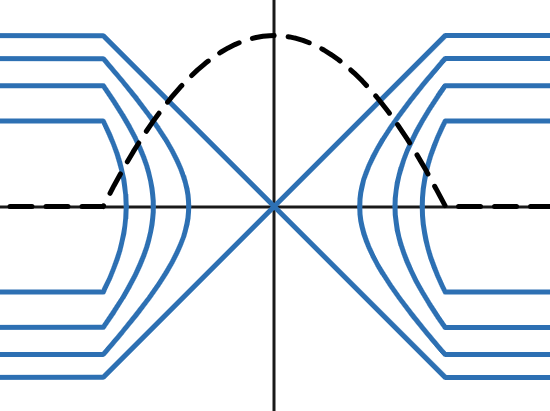
\includegraphics[width=0.3\textwidth]{classical-trajectories.png}
    \caption{Classical Phase space trajectories for the barrier potential $\varphi(x) = -\frac{1}{2}\omega^2x^2$} for the energies $E = 0.25\varphi_{max}, 0.5\varphi_{max}, 0.75\varphi_{max},$ and $\varphi_{max}$. The plot with $E = \varphi_{max}$ is the one that passes through the center.  The dotted line is $V(x)$.
    \label{fig:phase_space_barrier}
\end{figure}
\subsection{Imaginary time trajectories with energy below the barrier}
Adding the imaginary time trajectory connecting the two parts, it will correspond to moving in imaginary time, which is equivilant to switching the order of the terms in the square root in equation \ref{eq:classical-momentum}:
\begin{equation}
    \label{eq:imaginary-time-momentum}
    p = \pm 2m\sqrt{V(x) - E}
\end{equation}
giving the red plots in figure \ref{fig:phase_space_barrier_with_tunneling}.
\begin{figure}[h]
    \centering
    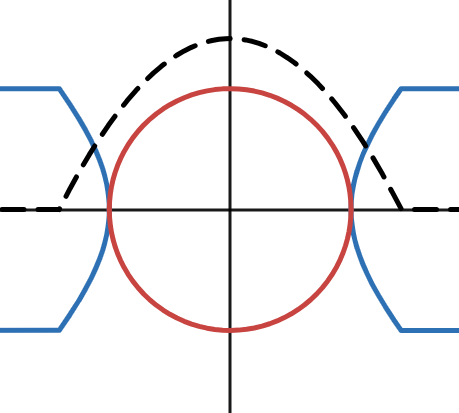
\includegraphics[width=0.3\textwidth]{classical-trajectories-with-tunneling.png}
    \caption{Classical Phase space trajectories for the barrier potential $\varphi(x) = -\frac{1}{2}\omega^2x^2$} for the energy $E = 0.5\varphi_{max}$ including motion in an imaginary time. The red line is the imaginary time trajectories connecting the two sides of the barrier. The dotted line is $V(x)$.
    \label{fig:phase_space_barrier_with_tunneling}
\end{figure}
It is clear to see in figure \ref{fig:phase_space_barrier_with_tunneling} that the instanton trajectory connects to the two classical trajectories at $x = a$ and $x = b$, the points at whcih $E = V(x)$ on the two sides of the barrier, where the square roots in both equation \ref{eq:classical-momentum} and \ref{eq:imaginary-time-momentum} are zero. In these trajectories, the particle starts from one side and ends on the other side of the barrier, with the real part of its momentum starting and finishing with the same value.
\subsection{Classical trajectories with energy above the barrier}
The classical trajectories for particles moving with $E > V_{max}$ can be seen in figure \ref{fig:phase_space_above_barrier}.
\begin{figure}[h]
    \centering
    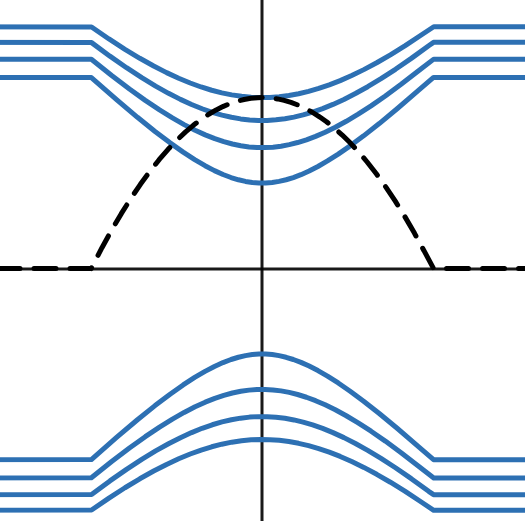
\includegraphics[width=0.3\textwidth]{classical-trajectories-above-barrier.png}
    \caption{Classical Phase space trajectories for the barrier potential $\varphi(x) = -\frac{1}{2}\omega^2x^2$} for the energies $1.25\varphi_{max}, 1.5\varphi_{max}, 1.75\varphi_{max},$ and $2\varphi_{max}$. The dotted line is $V(x)$.
    \label{fig:phase_space_above_barrier}
\end{figure}
One can see that in each side of the barrier there are two distinct trajectories with opposite momenta that do not interest. In other words, for every 2 points $x_i$ and $x_f$ on the same side of the barrier, there are two differet paths with $p = \pm2m\sqrt{E - V}$ that connecte them. This means that the classical trajectories do not contain any option for reflection.
\subsection{Instantons in trajectories with energy above the barrier}
Intuitivly, we can think about an instanton that will connect that two seperate trajectories in the same way the instanton allowed the particle to tunnel through the barrier. Since momentum is never zero, the instanton will have to flip it, and thus the most logical place to put it is along the $p$ axis. The suggested trajectory can be seen in figure \ref{fig:phase_space_above_barrier_with_tunneling}.
\begin{figure}[h]
    \centering
    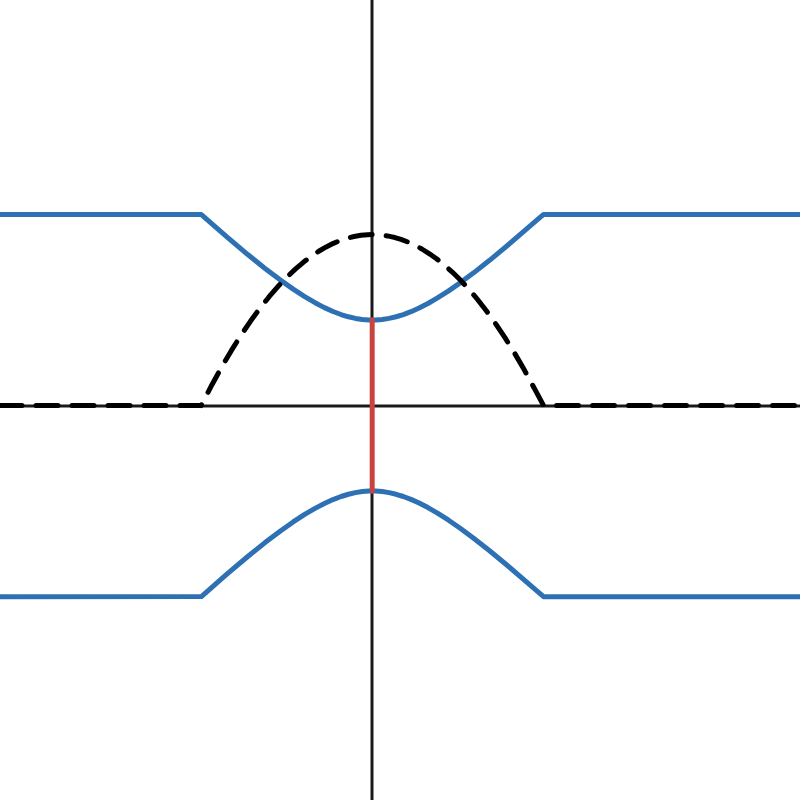
\includegraphics[width=0.3\textwidth]{classical-trajectories-above-barrier-with-tunneling.png}
    \caption{Classical Phase space trajectories for the barrier potential $\varphi(x) = -\frac{1}{2}\omega^2x^2$} for the energy $1.25\varphi_{max}$ including motion in an imaginary time. The red line is the imaginary time trajectory connecting the two oppposite-p trajectories. The dotted line is $V(x)$.
    \label{fig:phase_space_above_barrier_with_tunneling}
\end{figure}
\subsection{Green functions}
In this and the following section, we will assume, for the sake of simplicity and without loss of generality, that the potential is maximized for $x = 0$. For every trajectory $(n)$:
\begin{equation}
    G^{(n)}(x_i, x_f; E) \approx \frac{m}{i\hbar}\frac{1}{\left|\sqrt{p(x_i)p(x_f)}\right|}\exp(\frac{i}{\hbar}\int_{x_i}^{x_f}p(x)dx)
\end{equation}
with the integral in the exponent going along the trajectory path. For every trajectory, the path starts by moving from $x_i$ to $0$ with momentum $p_i$ and ends by moving back from $0$ to $x_f$ which is one the same side as $x_i$, and with an opposite momentum $p_f = -p_i$.
\newline
In the middle of the trajectory $G^{(n)}$ there are $2n+1$ passages through the complex plane in both $p$ and $x$. In the complex $p$ plane, in order to change the momentum from $p_i$ to $p_f$, it will move along the semicircle with a constant $|p|$. In the complex $x$ plane, it will have to pass through a branch cut in the momentum $p = \pm2m\sqrt{E - V(x)}$ to get the phase in the momentum. So, naming the closest point on the barnch cut $x_c$, the trajectory moves from $0$ to the $x_c$ and back:
\begin{equation}
    G^{(n)}(x_i, x_f; E) \approx \frac{m}{i\hbar}\frac{1}{\left|\sqrt{p(x_i)p(x_f)}\right|}\exp(\frac{i}{\hbar}\left(
        \int_{x_i}^{0}p(x)dx +
        i (4n + 2) \int_{0}^{x_c}|p(x)|dx + 
        \int_{0}^{x_f}p(x)dx
    \right))
\end{equation}
\subsection{The Tunneling action}
The action that we got in the exponent is very similar to the action for tunneling:
\begin{equation}
    S[x] = \frac{i}{\hbar}\left(
        \int_{x_i}^{0}p(x)dx +
        i (4n + 2) \int_{0}^{x_c}|p(x)|dx + 
        \int_{0}^{x_f}p(x)dx
    \right)
\end{equation}
Using integrtion by parts on all three integrals gives
\begin{equation}
    S[x] = \frac{i}{\hbar}\left(
        \left[xp\right]_{x_i}^{x_f} -
        \int_{p_i}^{0}x(p)dp -
        i (4n + 2) \int_{0}^{\pi}|x(p)|^2d\varphi - 
        \int_{0}^{x_f}x(p)dp
    \right)
\end{equation}
Where the central integral became an integral along the semicircle in the complex p plane. Which means we can think about it as tunneling along the p axis, jumping from positive momentum to negative momentum in the same way that the trajectories in under the bearier tunnling jump from $a$ to $b$.
\end{document}